\section{Interactive Visualization Strategies}

\subsection{Navigation Strategies}

Interactive data visualization systems have a basic requirement which is to enable navigation of large information. Navigation techniques allow the user to move between different levels of detail in the data. Zooming and panning, overview1detail, and focus1context are the three main approaches that enable data visualization navigation. These techniques are applied instead of the detail-only approach that was introduced by the Keyhole problem to overcome the big data visualization complexities which may disorient the user due to the absence of an overview of the large information space \cite{salvendy2012handbook}. Attempts to compare the three approaches are inconclusive and subject to specific design scenarios, data, and user tasks however, experimental results demonstrate the superior performance of these navigation strategies over the detail-only strategy \cite{hornbaek2002navigation}.

\subsubsection{Zoom and Pan}

Zoom and pan operations when used in data visualization allow the user first to see the overview and then to interactively zoom into the data and pan the viewpoint within the data space to access details of interest. Zooming could be implemented using continuous space navigation as the Pad11 system \cite{bederson1994pad++} provide or to systematically access different scales as with the TreeMap system \cite{johnson1999tree}. The ability to zoom in to details of interest from an overview and zoom out to see the overview and the whole idea again is the main advantage of this approach. Maps are an example of the use of this approach but although how efficiently this approach uses screen apace and offers infinite scalability, users may become disoriented and lost when zooming in and panning around the data space, since the overview is not shown also this approach can result in slower navigation because the intensive use of memory if not used correctly \cite{salvendy2012handbook}. 

\begin{figure}[h]
\begin{subfigure}{.5\textwidth}
  \centering
  \captionsetup{justification=centering}
  % include first image
  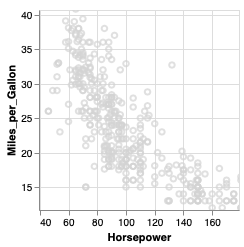
\includegraphics[width=.8\linewidth]{Report-latex/tex_files/pics/zoom1.png}  
  \caption{Before the Zoom (Vega-Lite website)}
  \label{fig:sub-first}
\end{subfigure}
\begin{subfigure}{.5\textwidth}
  \centering
  \captionsetup{justification=centering}
  % include second image
  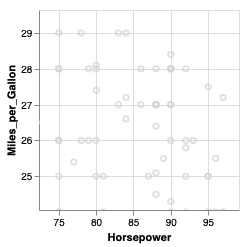
\includegraphics[width=.8\linewidth]{Report-latex/tex_files/pics/zoom2.png}  
  \caption{After the Zoom (Vega-Lite website)}
  \label{fig:sub-second}
\end{subfigure}
\captionsetup{justification=centering}
\caption{Zoom example }
\label{fig:fig}
\end{figure}

\subsubsection{Overview \& Detail}

The overview1 \& detail strategy enables multiple views to display both an overview and a detail view simultaneously. Unlike the zoom \& pan strategy, the overview \& detail strategy preserves the context of the whole data set while allowing the user to examine detailed information about a particular part of interest. This strategy is often used in both map and image viewing systems \cite{plaisant1995image} and different applications combined with zoom \& pan strategy like in maps. One issue with this strategy is that even though it enables multiple views, usually the detailed view consumes the display area, especially on small screens, and left the overview not fully clear.

\begin{figure}[H]
\centering
\captionsetup{justification=centering}
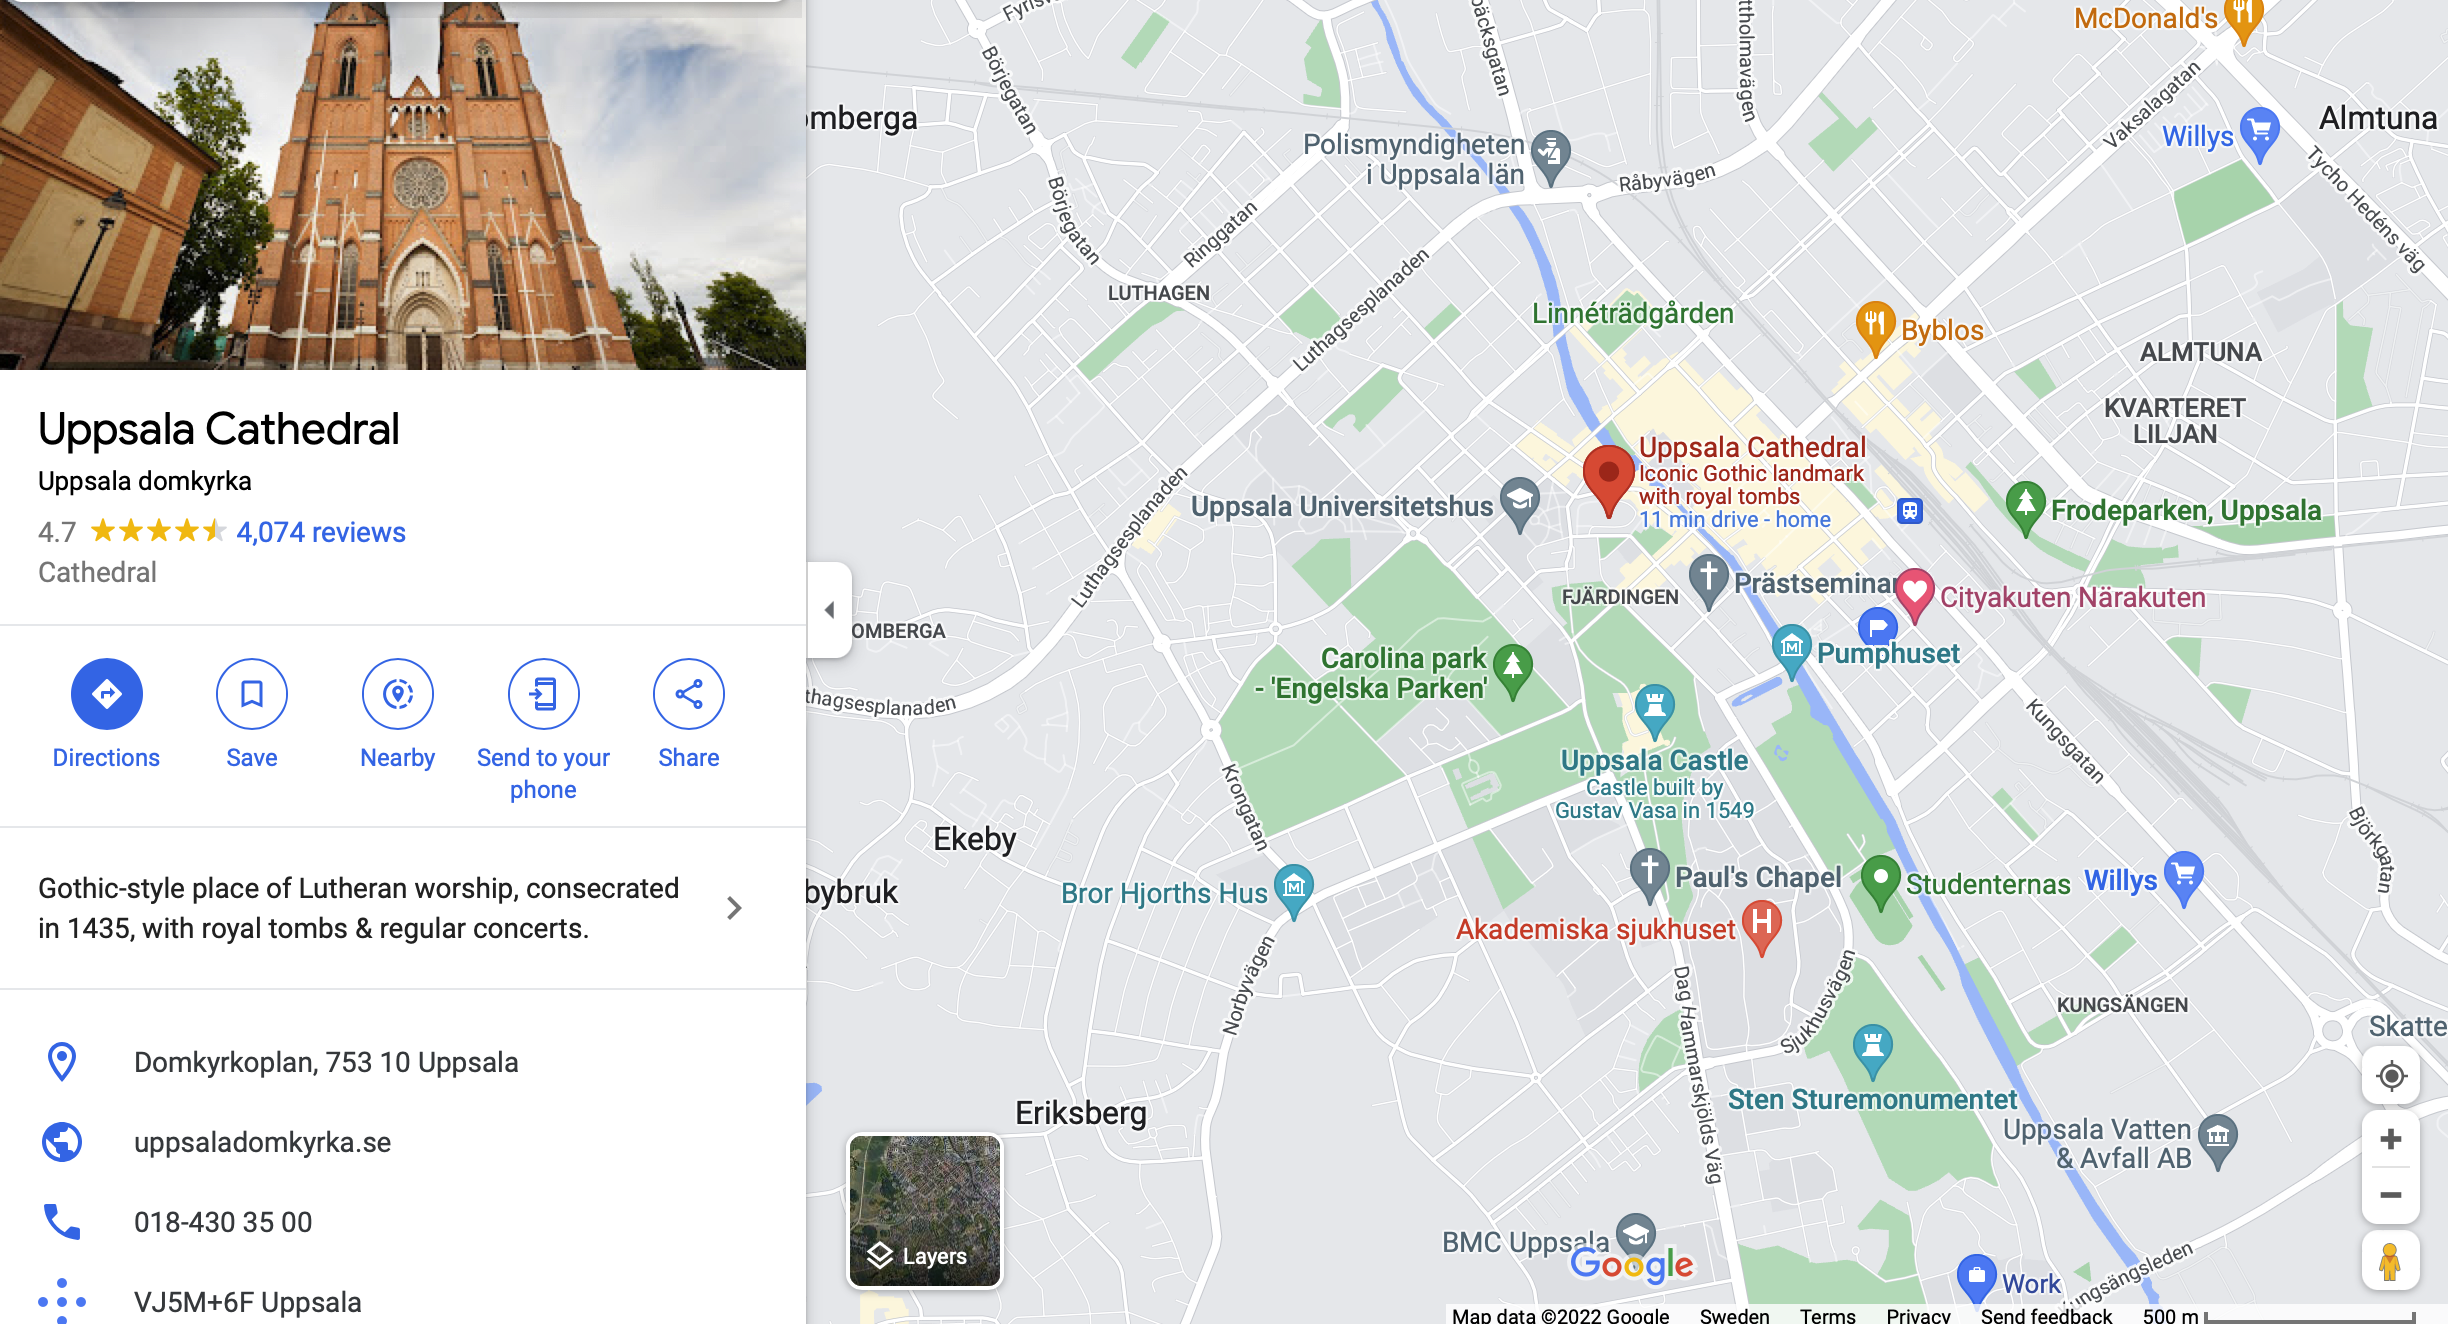
\includegraphics[width=0.9\textwidth]{Report-latex/tex_files/pics/over.png}
\caption{Overview \& Detail (Google map)}
\end{figure}

\subsubsection{Focus \& Context}

Instead of creating a separate view for the intended region of the overview, the focus \& context strategy allows the focus region to grow and differentiate itself from the rest of the overview area. The focus region can show additional information by getting expanded and magnified while the overview gets partially compressed to allow for such expansion in the focus area. The bifocal display is one of the variations of the focus \& context strategy which uses two levels of magnification and the concept of the bifocal display is used in TableLens \cite{rao1994table} and the dock of application icons in desktop operating systems. This strategy provides continuity of detail within the context of the overview however, this strategy applies some distortion to the overview to put more focus on the intended part which might cause some disorientation to the users \cite{baudisch2002keeping}. Moreover, this technique has limited scalability typically under a 10:1 zoom factor \cite{salvendy2012handbook}

\begin{figure}[h]
\begin{subfigure}{.5\textwidth}
  \centering
  \captionsetup{justification=centering}
  % include first image
  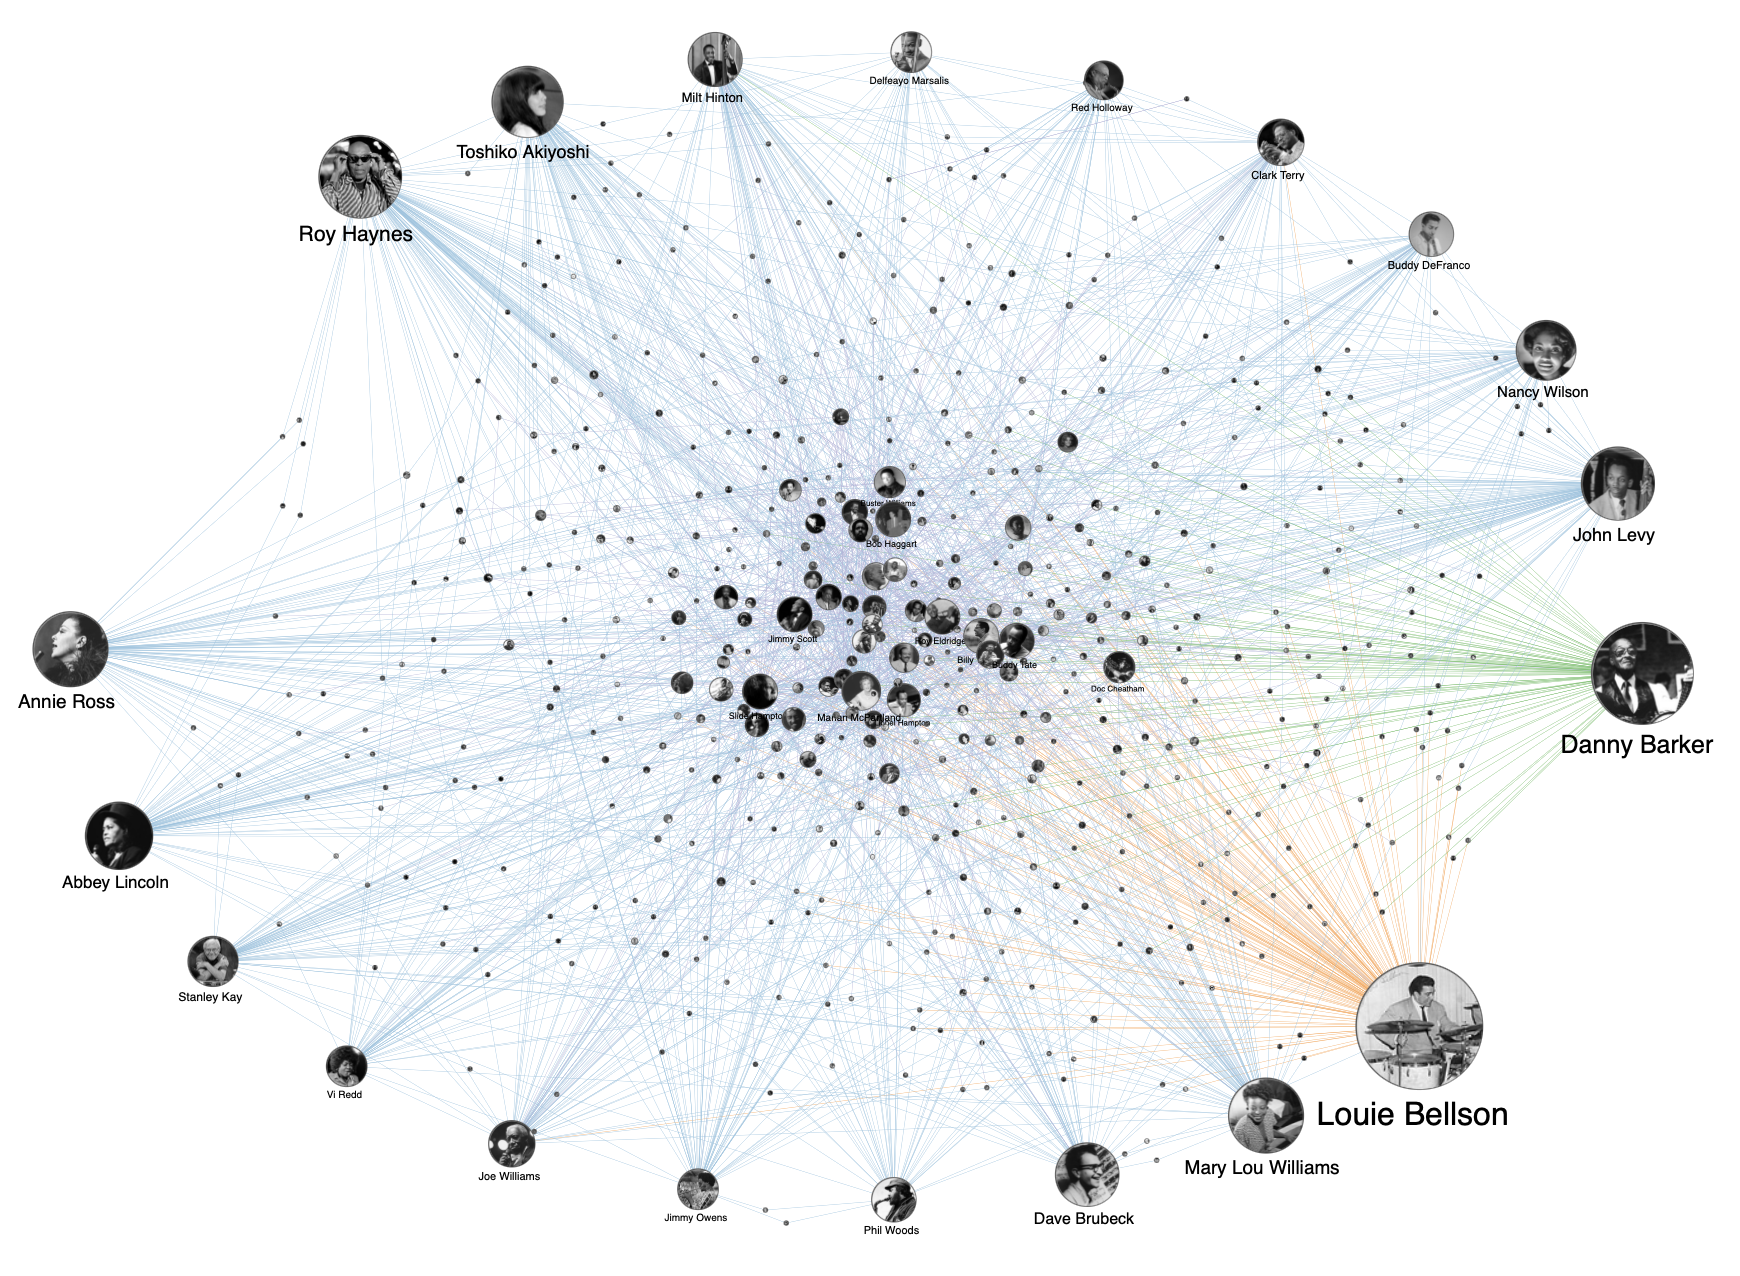
\includegraphics[width=.8\linewidth]{Report-latex/tex_files/pics/f1.png}  
  \caption{The Overview Visualisation}
  \label{fig:sub-first}
\end{subfigure}
\begin{subfigure}{.5\textwidth}
  \centering
  \captionsetup{justification=centering}
  % include second image
  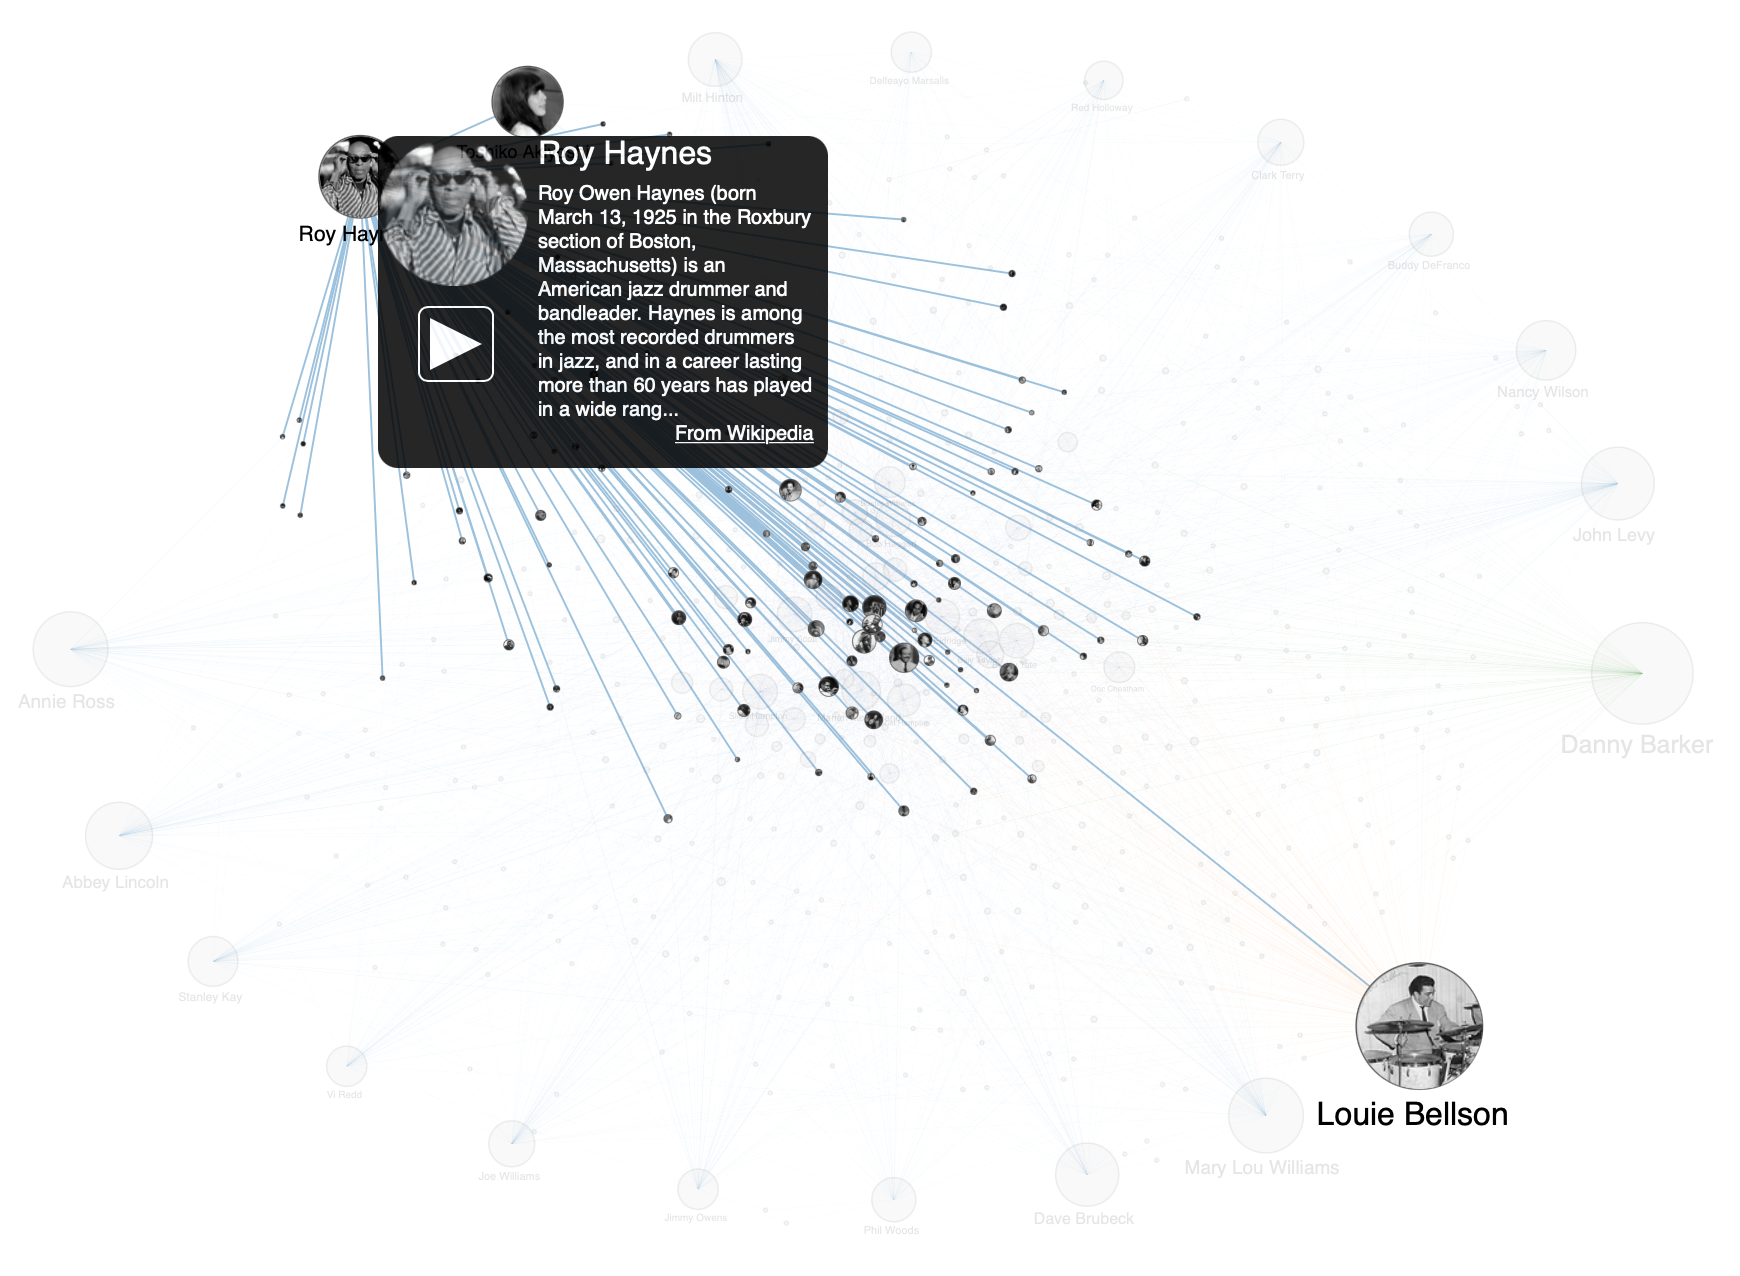
\includegraphics[width=.8\linewidth]{Report-latex/tex_files/pics/f2.png}  
  \caption{Focus Region}
  \label{fig:sub-second}
\end{subfigure}
\captionsetup{justification=centering}
\caption{Focus \& Context (https://linkedjazz.org/network/) }
\label{fig:fig}
\end{figure}

\subsection{Visual Interaction Strategies}

While most navigation strategies have issues with scalability, Visual interaction strategies support scalability and it is more of user-centered techniques. These techniques allow the user to access alternative perspectives and insights since for even modest data volumes it is impossible to show all the data. There are many interactions techniques for data visualizations \cite{ward2015interactive} and here are the main four categories that should be considered in the design of visualization systems.

\subsubsection{Selecting}

For a huge data set that can be divided into multiple groups or subsets, The capability to interactively select items of interest in visualization is fundamental. Grouping similar items into a set, selecting items, adding items to a selection, removing selected items, and completely clear selection are achievable actions using selection techniques. A user can select items using direct or indirect actions. Direct selection can be implemented in many different ways, such as pointing at the item using the mouse and dragging it to join a group of items \cite{wills1996selection}. On the other hand, Indirect selection criteria are based on a set of constraints that user specifies their ranges of values. For example, selecting graph nodes with a user-defined distance from another node \cite{ward2015interactive}. Selection is like stroking visual objects with an artist’s brush and that is why it is usually referred to as brushing.


\subsubsection{Linking}

When selection is made in one view, linking is used to dynamically relate information between multiple views \cite{north2001multiple,wang2000guidelines}. Selecting (brushing) and linking is the most common view coordination strategy and it is usually called linked brushing \cite{becker1987brushing}. With this strategy, selected items in one view are also highlighted in other views which enable users to uncover relationships and construct comprehensive understandings of the data set. Moreover, linked brushing allows users to define complex constraints by optimizing each view to specify constraints on certain data types and degrees of accuracy \cite{ward2015interactive}. For example, by specifying temporal constraints with a timeline visualization and geographic constraints with a map. Linking strategy comes with a diverse range of options for connection between different linked views such as unlinking one view of the data to explore other regions or specifying what type of information is communicated. 

\begin{figure}[H]
\centering
\captionsetup{justification=centering}
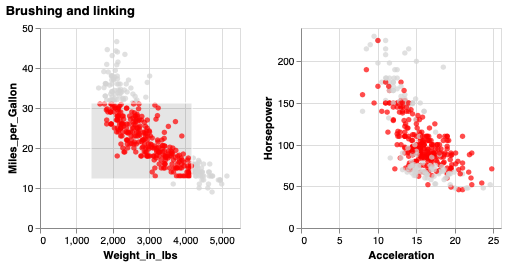
\includegraphics[width=0.9\textwidth]{Report-latex/tex_files/pics/brlink2.png}
\caption{Selecting (brushing) \& Linking (Vega-lite website)}
\end{figure}


\subsubsection{Filtering}

One of the main strategies to deal with a huge data set is by using interactive filtering operations which reduce the quantity of data visualized and focus on interesting features. Dynamic query filters provide rapid feedback, reduce the quantity of information, and permit exploration of the relationships between attributes. Visual widgets are used to assign a range of interests and view the filtered results in the visualization. There is a diffusion between selecting and filtering however there is a thin but important distinction between them. Filtering is usually achieved through a separate interface and via indirect action. Also, filtering can be executed before viewing large data set to avoid overwhelming the system. On the other hand, selecting is usually achieved via direct action, such as mouse clicks. Even though selecting and filtering strategies have different mechanisms but the outcome of both of them on the view can be indistinguishable \cite{ward2015interactive}.

\subsubsection{Rearranging and Remapping}

It is important users have the ability to customize the visual mapping form rather than having a single configuration that might be inadequate. Since the spatial layout is the most important visual mapping, rearranging the spatial layout of the information is very effective for revealing new insight. A simple operation but important as it gives the user the flexibility to explore relationships between different attributes and finds what best suits their needs.